\documentclass[a4paper, final]{article}
\usepackage[14pt]{extsizes} 
\usepackage[T2A]{fontenc}
\usepackage[utf8]{inputenc}
\usepackage[russian]{babel}
\usepackage{amsmath}
\usepackage{subfig}
\usepackage[left=25mm, top=20mm, right=20mm, bottom=20mm, footskip=10mm]{geometry}
\usepackage{ragged2e} 
\usepackage{setspace}
\usepackage{stackengine}
\usepackage{indentfirst} 
\usepackage{moreverb} 
\renewcommand\verbatimtabsize{4\relax}
\renewcommand\listingoffset{0.2em} 
\renewcommand{\arraystretch}{1.4} 
\usepackage[font=small, singlelinecheck=false, justification=centering, format=plain, labelsep=period]{caption} 
\usepackage{listingsutf8}
\usepackage{xcolor} 
\usepackage{listings}
\usepackage{hyperref}
\usepackage{enumitem} 
\usepackage{verbatim}
\usepackage{tikz} 
\usepackage{amssymb}
\usepackage{pdflscape} %для pdf
\usepackage{pdfpages} %для pdf
\usepackage{graphicx}
\usepackage{tabularx}
\usepackage{multirow}
\usepackage{cmap}
\usepackage{float}

\graphicspath{ {./Рисунки/} }
\setlist[enumerate,itemize]{leftmargin=1.2cm} %отступ в перечислениях

\hypersetup{colorlinks,
  allcolors=[RGB]{061 087 255}}

\lstloadlanguages{ [LaTeX] TeX}

\lstset{language =[LaTeX] TeX, 
extendedchars=true , 
escapechar = | , 
frame=tb , 
commentstyle=\itshape , 
stringstyle =\bfseries}

\textheight=24cm 
\textwidth=16cm
\oddsidemargin=0pt 
\topmargin=-1.5cm
\parindent=24pt 
\parskip=0pt 
\tolerance=2000 
\flushbottom



\begin{document} 
\newcommand{\specialcell}[2][l]{\begin{tabular}[#1]{@{}l@{}}#2\end{tabular}}
\lstset{
  language=SQL, % Язык кода по умолчанию
  morekeywords={*,...}, % если хотите добавить ключевые слова, то добавляйте
  % Цвета
  keywordstyle=\color{keyword}\ttfamily\bfseries,
  %stringstyle=\color{string}\ttfamily,
  stringstyle=\ttfamily\color{red!50!brown},
  commentstyle=\color{comment}\ttfamily,
  morecomment=[l][\color{morecomment}]{\#},
  % Настройки отображения
  breaklines=true, % Перенос длинных строк
  basicstyle=\ttfamily\footnotesize, % Шрифт для отображения кода
  backgroundcolor=\color{bk}, % Цвет фона кода
  frame=single,xleftmargin=\fboxsep,xrightmargin=-\fboxsep, % Рамка, подогнанная к заголовку
  rulecolor=\color{frame}, % Цвет рамки
  tabsize=3, % Размер табуляции в пробелах
  % Настройка отображения номеров строк. Если не нужно, то удалите весь блок
  numbers=left, % Слева отображаются номера строк
  stepnumber=1, % Каждую строку нумеровать
  numbersep=5pt, % Отступ от кода
  numberstyle=\small\color{black}, % Стиль написания номеров строк
  % Для отображения русского языка
  extendedchars=true,
  literate={Ö}{ {\"O} }1
  {~}{ {\textasciitilde} }1
  {а}{ {\selectfont\char224} }1
  {б}{ {\selectfont\char225} }1
  {в}{ {\selectfont\char226} }1
  {г}{ {\selectfont\char227} }1
  {д}{ {\selectfont\char228} }1
  {е}{ {\selectfont\char229} }1
  {ё}{ {\"e} }1
  {ж}{ {\selectfont\char230} }1
  {з}{ {\selectfont\char231} }1
  {и}{ {\selectfont\char232} }1
  {й}{ {\selectfont\char233} }1
  {к}{ {\selectfont\char234} }1
  {л}{ {\selectfont\char235} }1
  {м}{ {\selectfont\char236} }1
  {н}{ {\selectfont\char237} }1
  {о}{ {\selectfont\char238} }1
  {п}{ {\selectfont\char239} }1
  {р}{ {\selectfont\char240} }1
  {с}{ {\selectfont\char241} }1
  {т}{ {\selectfont\char242} }1
  {у}{ {\selectfont\char243} }1
  {ф}{ {\selectfont\char244} }1
  {х}{ {\selectfont\char245} }1
  {ц}{ {\selectfont\char246} }1
  {ч}{ {\selectfont\char247} }1
  {ш}{ {\selectfont\char248} }1
  {щ}{ {\selectfont\char249} }1
  {ъ}{ {\selectfont\char250} }1
  {ы}{ {\selectfont\char251} }1
  {ь}{ {\selectfont\char252} }1
  {э}{ {\selectfont\char253} }1
  {ю}{ {\selectfont\char254} }1
  {я}{ {\selectfont\char255} }1
  {А}{ {\selectfont\char192} }1
  {Б}{ {\selectfont\char193} }1
  {В}{ {\selectfont\char194} }1
  {Г}{ {\selectfont\char195} }1
  {Д}{ {\selectfont\char196} }1
  {Е}{ {\selectfont\char197} }1
  {Ё}{ {\"E} }1
  {Ж}{ {\selectfont\char198} }1
  {З}{ {\selectfont\char199} }1
  {И}{ {\selectfont\char200} }1
  {Й}{ {\selectfont\char201} }1
  {К}{ {\selectfont\char202} }1
  {Л}{ {\selectfont\char203} }1
  {М}{ {\selectfont\char204} }1
  {Н}{ {\selectfont\char205} }1
  {О}{ {\selectfont\char206} }1
  {П}{ {\selectfont\char207} }1
  {Р}{ {\selectfont\char208} }1
  {С}{ {\selectfont\char209} }1
  {Т}{ {\selectfont\char210} }1
  {У}{ {\selectfont\char211} }1
  {Ф}{ {\selectfont\char212} }1
  {Х}{ {\selectfont\char213} }1
  {Ц}{ {\selectfont\char214} }1
  {Ч}{ {\selectfont\char215} }1
  {Ш}{ {\selectfont\char216} }1
  {Щ}{ {\selectfont\char217} }1
  {Ъ}{ {\selectfont\char218} }1
  {Ы}{ {\selectfont\char219} }1
  {Ь}{ {\selectfont\char220} }1
  {Э}{ {\selectfont\char221} }1
  {Ю}{ {\selectfont\char222} }1
  {Я}{ {\selectfont\char223} }1
  {\{}{ { {\color{brackets}\{} } }1 % Цвет скобок {
  {\} }{ { {\color{brackets}\} } } }1 % Цвет скобок }
}
\thispagestyle{empty}
\begin{center}
\hfill \break
\hfill \break
\normalsize{МИНИСТЕРСТВО НАУКИ И ВЫСШЕГО ОБРАЗОВАНИЯ РОССИЙСКОЙ ФЕДЕРАЦИИ\\
 федеральное государственное автономное образовательное учреждение высшего образования «Санкт-Петербургский политехнический университет Петра Великого»\\[10pt]}
\normalsize{Институт компьютерных наук и кибербезопасности}\\[10pt] 
\normalsize{Высшая школа технологий искусственного интеллекта}\\[10pt] 
\normalsize{Направление: 02.03.01 Математика и компьютерные науки}\\

\hfill \break
\hfill \break
\hfill \break
\large{Отчёт по по дисциплине}\\
\large{<<Курсовое проектирование по управлению ресурсами суперэвм>>}\\
\large{Решение задачи нахождения алгебраических дополнений элементов матрицы}\\
\hfill \break
\vspace{2cm}


\end{center}
 
\small{ 
\begin{tabular}{lrrl}
\!\!\!Студент, & \hspace{2cm} & & \\
\!\!\!группы 5130201/20102 & \hspace{2cm} & \underline{\hspace{3cm}} &Салимли А. М. \\\\
\!\!\!Преподаватель & \hspace{2cm} & \underline{\hspace{3cm}} & Курочкин М. А. \\\\
&&\hspace{5cm}
\end{tabular}
\begin{flushright}
<<\underline{\hspace{1cm}}>>\underline{\hspace{2.5cm}} 2025г.
\end{flushright}
}
\hfill \break

\begin{center} \small{Санкт-Петербург, 2025} \end{center}
\thispagestyle{empty} 

\newpage
\tableofcontents
\newpage
\section*{Введение}
\addcontentsline{toc}{section}{Введение}
Многие задачи, возникающие на практике, требуют большого объема вычислений. Одним из вариантов решения сложных вычислительных задач является использование
параллельного программирования.
За последние несколько десятилетий стало очень распространено вычисление с помощью графических ускорителей — устройств с массивно-параллельной архитектурой.
Производить вычисления общего назначения можно на видеокартах архитектуры Nvidia
CUDA.
Сегодня спроектированы и испытаны многие компьютеры, которые используют в своей
архитектуре тот или иной вид параллельной обработки данных. Сложность работы
программирования заключается в координации используемых ресурсов.
Одним из примеров массивных вычислительных систем является суперкомпьютерный
центр «Политехнический». Часть узлов этого суперкомпьютера оборудована графическими ускорителями Nvidia Tesla K40X.


\newpage
\section{Постановка задачи}

\subsection{Задачи лабораторной работы}

В рамках данной работы необходимо изучить технологию параллельного программирования с использованием архитектуры Nvidia CUDA.

Также необходимо ознакомиться с принципом использования ресурсов суперкомпьютерного центра «Политехнический» для решения прикладной задачи.

Необходимо написать программу для решения поставленной задачи с использованием
технологии Nvidia CUDA и провести исследование зависимости времени выполнения
программы от количества используемых ресурсов.

В рамках курсовой работы необходимо написать программу для подсчета алгебраических дополнений заданной матрицы. 


\newpage

\section{Аппаратно-программная платформа NVIDIA CUDA}
    \subsection{Архитектура NVIDIA CUDA}
    Архитектура NVIDIA CUDA (Compute Unified Device Architecture) - это программная и аппаратная платформа, разработанная компанией NVIDIA, которая позволяет использовать графические процессоры (GPU) для параллельных вычислений и ускорения обработки данных \cite{cuda_tech}.
    
    Основной принцип архитектуры CUDA заключается в использовании мощности вычислений графического процессора для выполнения параллельных задач, работающих вместе с центральным процессором (CPU) компьютера. Графический процессор состоит из множества вычислительных ядер, которые могут выполнять однотипные задачи одновременно, независимо друг от друга. Это позволяет обрабатывать большие объемы данных и решать сложные вычислительные задачи с высокой производительностью.
    
    Основные характеристики архитектуры NVIDIA CUDA:
    \begin{itemize}
        \item Язык программирования: CUDA поддерживает язык программирования CUDA C/C++, который предоставляет расширения для работы с параллельными вычислениями на GPU. 
        \item Модель исполнения: CUDA использует модель исполнения, основанную на понятии ядер (kernels). Ядро (kernel) - это функция, которая выполняется параллельно на множестве потоков на графическом процессоре.
        \item Модель памяти: CUDA предоставляет шесть типов памяти, включая глобальную память, разделяемую память (shared memory) и константную память (constant memory). Каждый тип памяти имеет свои особенности и используется для различных целей, таких как обмен данными между потоками и сохранение постоянных данных.
    \end{itemize}
    \subsection{Вычислительные возможности NVIDIA CUDA}
    Параметр "compute capability"\,(вычислительная способность) в NVIDIA CUDA используется для описания возможностей и характеристик конкретной архитектуры графического процессора \cite{cuda_guide}. Он определяет, какие функции и возможности доступны для программ, компилируемых с использованием CUDA.
    
    Вычислительная способность обозначается числовым значением, состоящим из двух цифр, разделенных точкой (например, 6.1 или 7.0). Первая цифра обозначает основную версию архитектуры, а вторая цифра указывает на подверсию.
    
    Вычислительная способность зависит от конкретной архитектуры GPU и определяет следующие характеристики:
    \begin{itemize}
        \item Количество и тип вычислительных ядер: Вычислительная способность определяет количество ядер SM (Streaming Multiprocessors) на графическом процессоре и тип архитектуры ядра, такой как NVIDIA's Fermi, Kepler, Maxwell, Pascal, Volta, Turing или Ampere. Каждая архитектура имеет свои особенности и функции.
        \item Размер разделяемой памяти и регистров: Вычислительная способность также определяет доступный объем разделяемой памяти (shared memory) и количество доступных регистров для каждого потока выполнения на графическом процессоре. Эти ресурсы могут использоваться для ускорения вычислений и обмена данными между потоками.
        \item Поддержка определенных функций и инструкций: Вычислительная способность определяет, какие функции и инструкции доступны для использования в программе CUDA. Новые архитектуры могут включать новые инструкции и возможности, которые не доступны в старых версиях.
        \item Производительность и энергоэффективность: Вычислительная способность также связана с производительностью и энергоэффективностью архитектуры GPU. Более новые версии архитектур часто имеют улучшенную производительность и более эффективное использование энергии.
    \end{itemize}
    
    В СК «Политехник - РСК Торнадо», на котором проводились вычисления, установлены графические процессоры Nvidia Tesla K40. Они имеют compute capability версии 3.5, ниже приведены их основные характеристики.
    \begin{itemize}
    \item Количество одновременно выполняющихся ядер: 32;
    \item Максимальная размерность сетки блоков: 3-х мерная;
    \item Максимальная x-составляющая сетки блоков: $2^{31 - 1}$;
    \item Максимальная y- и z-составляющая сетки блоков: 65535;
    \item Максимальная размерность блока: 3-х мерный;
    \item Максимальная x- и y-составляющая блока: 1024;
    \item Максимальная z-составляющая блока: 64;
    \item Максимальное количество нитей в блоке: 1024;
   \end{itemize}
    \subsection{Потоковая модель}
    Вычислительная архитектура CUDA основана на концепции одна команда на множество данных (Single Instruction Multiple Data, SIMD) и понятии мультипроцессора.
    
    Концепция \textbf{SIMD} подразумевает, что одна инструкция позволяет одновременно обработать множество данных. 
    
    \textbf{Мультипроцессор} — это многоядерный SIMD процессор, позволяющий в каждый определенный момент времени выполнять на всех ядрах только одну инструкцию. Каждое ядро мультипроцессора скалярное, т.е. оно не поддерживает векторные операции в чистом виде.
    
    Также в вычислительной архитектуре CUDA важны понятия устройство и хост.
    
    \textbf{Устройство (device)} - видеоадаптер, поддерживающий драйвер CUDA, или другое специализированное устройство, предназначенное для исполнения программ, использующих CUDA.
    
    
    \textbf{Хост (host)} - программа в обычной оперативной памяти компьютера, использующую CPU и выполняющую управляющие функции по работе с устройством.
    
    Логически устройство можно представить как набор мультипроцессоров (см. Рис. \ref{device}) плюс драйвер CUDA.
    
    \begin{figure}[h!]
    	\centering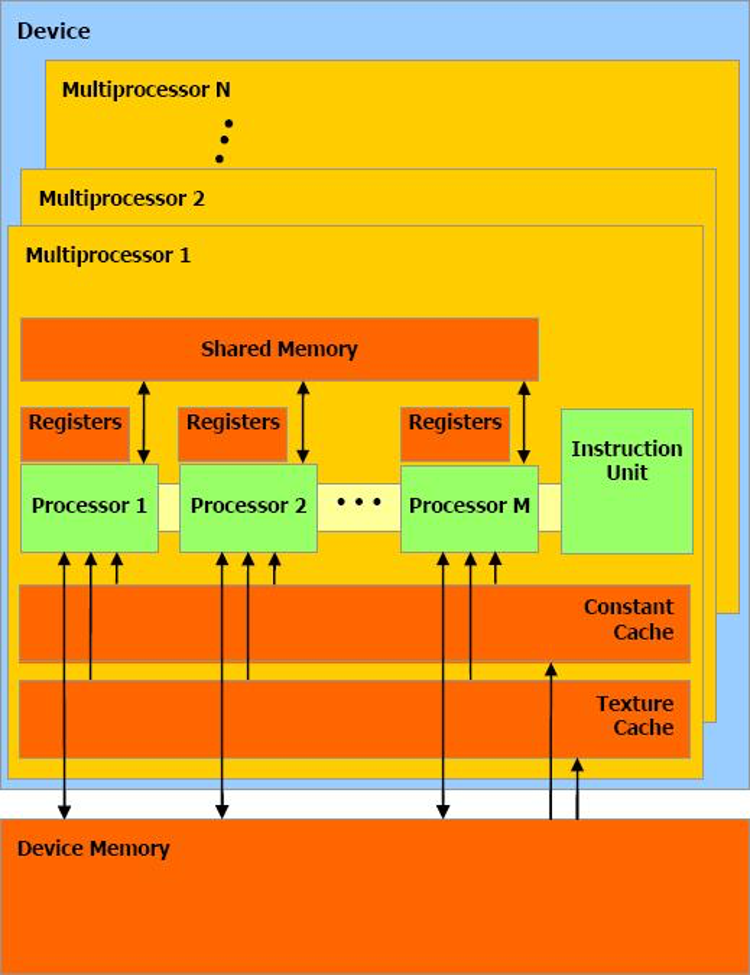
\includegraphics[scale=0.75]{logik.png}
         \caption{Архитектура устройства}	
     \label{device}
    \end{figure}

    \clearpage
    \subsection{Устройство памяти}
    В CUDA выделяют шесть видов памяти (рис. \ref{memory}). Это регистры, локальная, глобальная, разделяемая, константная и текстурная память.
    Такое обилие обусловлено спецификой видеокарты и первичным ее предназначением, а также стремлением разработчиков сделать систему как можно дешевле, жертвуя в различных случаях либо универсальностью, либо скоростью. Подробно каждый вид памяти будет рассмотрен в следующем разделе.
    \begin{figure}[h!]
    	\centering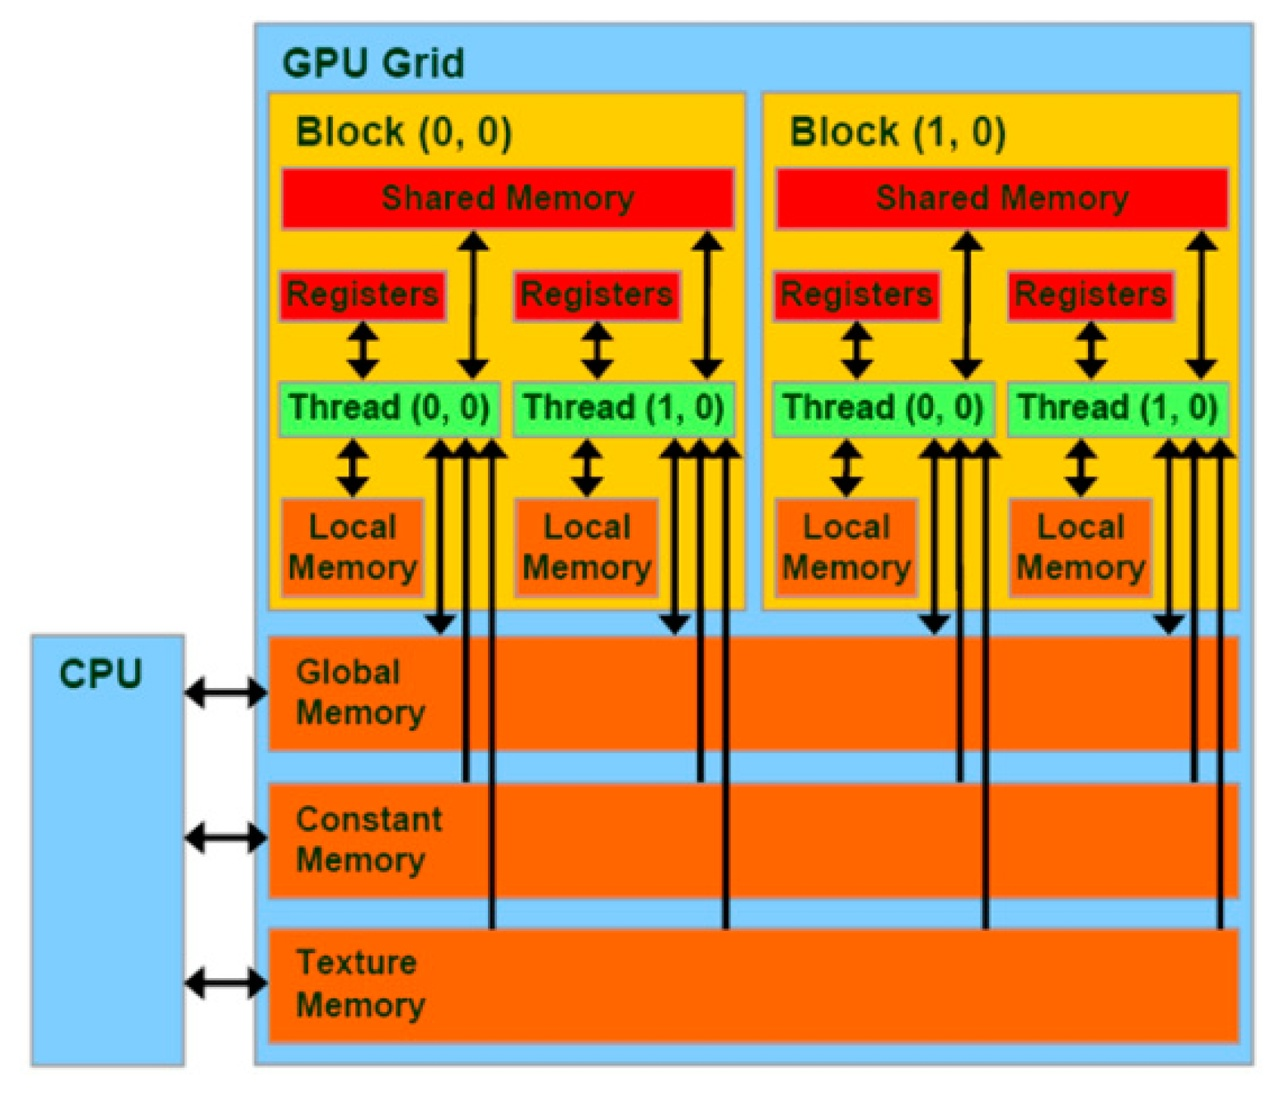
\includegraphics[scale=0.25]{memory.jpg}
         \caption{Виды памяти}	
     \label{memory}
    \end{figure}
    \subsection{Модели памяти}
    В CUDA выделяют шесть видов памяти:
    \begin{enumerate}
        \item \textbf{Регистры} -- память, в которой по возможности компилятор старается размещать все локальные переменные функций. Доступ к 
    таким переменным осуществляется с максимальной скоростью. В текущей архитектуре на один 
    мультипроцессор доступно 8192 32-разрядных регистра. 
    \item \textbf{Локальная память} --  в случаях, когда локальные данные процедур занимают слишком большой размер, или компилятор не может 
    вычислить для них некоторый постоянный шаг при обращении, он может поместить их в локальную память. Этому может способствовать, например, приведение указателей для типов разных размеров. Физически локальная память является аналогом глобальной памяти, и работает с той же скоростью.
    \item \textbf{Глобальная память} -- самый большой объём памяти, доступный для всех МП на видеочипе (размер от 256Mбайт до 4Гбайт). Основная особенность -  возможность 
    произвольной адресации. Однако глобальная память работает очень медленно, не кэшируется. Поэтому количество обращений к глобальной памяти следует минимизировать. Глобальная память необходима в основном для сохранения результатов работы программы перед отправкой 
    их на хост (в обычную память DRAM). 
    \item \textbf{Разделяемая память} -- некэшируемая, но быстрая память. Ее и рекомендуется использовать как 
    управляемый кэш. На один мультипроцессор доступно всего 16KB разделяемой памяти. 
    Отличительной чертой разделяемой памяти является то, что она адресуется одинаково для всех задач 
    внутри блока. Отсюда следует, что ее можно использовать для обмена данными между потоками 
    только одного блока.
    \item \textbf{Константная память} --  размер 
    составляет всего 64 Kбайт (на все устройство). Константная память кэшируется, поэтому доступ в общем случае достаточно быстрый. Кэш существует в единственном экземпляре для одного мультипроцессора, а значит, общий для всех задач внутри блока. 
    Константная память очень удобна в использовании. Можно размещать в ней данные любого типа и читать их 
    при помощи простого присваивания. Однако из-за её небольшого объема имеет смысл 
    хранить лишь небольшое количество часто используемых данных.
    \item \textbf{Текстурная память} --  блок памяти, доступный для чтения всеми МП. Кэшируется. Медленная, как глобальная - сотни тактов задержки при 
    отсутствии данных в кэше. Имеет очень важное свойство пространственной локальности. При вычислении на модели в виде матрицы, где соседние
    элементы взаимодействуют друг с другом, часто возникает необходимость обращаться к элементам окрестности элемента матрицы. С точки зрения адресной арифметики элементы окрестности какого-либо элемента матрицы не расположены в памяти рядом друг с другом. Для ускорения вычисления вышеописанного вида применяется текстурная память, которая позволяет кэшировать данные по свойству их пространственной, а не адресной локальности.
    \end{enumerate}
    \subsection{Модель вычислений на GPU}
    В основе модели вычислений на GPU лежит понятие сетки блоков.  На Рис. \ref{threads} ядро обозначено как Kernel. Все потоки, выполняющие это ядро, объединяются в блоки (Block), а блоки, в свою очередь, объединяются в сетку (Grid).

    \clearpage
    \begin{figure}[h!]
    	\centering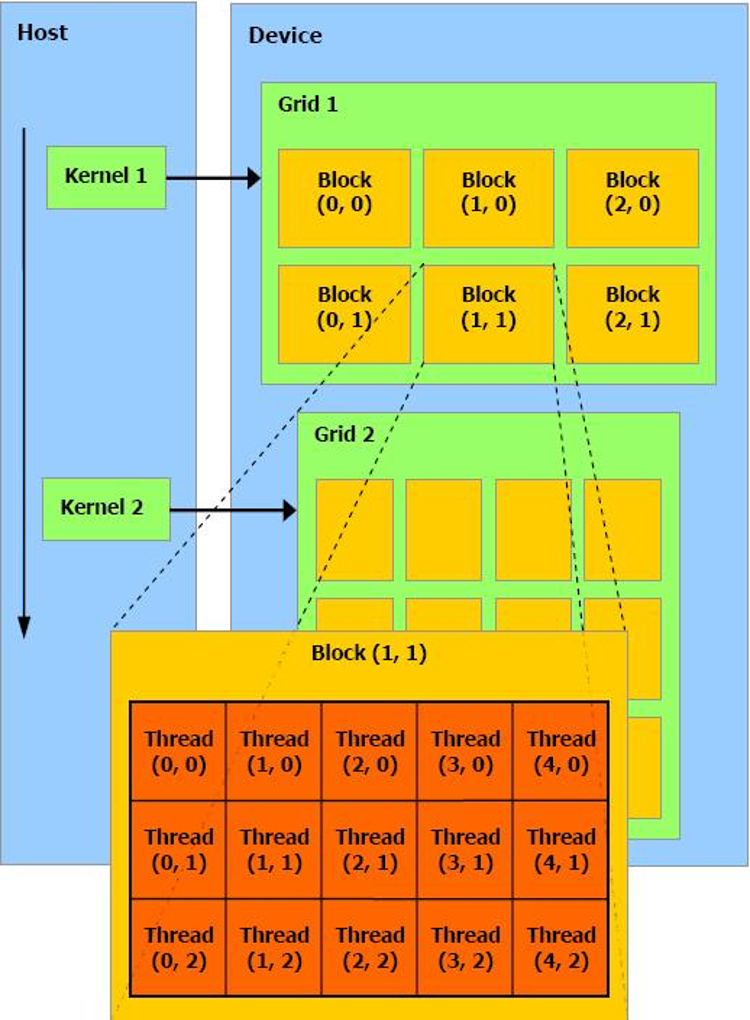
\includegraphics[scale=0.75]{threads.png}
         \caption{Организация потоков}	
     \label{threads}
    \end{figure}
    
    Вычисление шейдерной программы (ядра) на матрице данных распределяется по блокам, ответственным за отдельно взятый участок матрицы данных. Блоки образуют одно- двух- трёх мерную сетку.
    
    В свою очередь выполнение программы на участке матрицы данных блока выполняется параллельно в нитях, из которых состоит блок. Нить — это экземпляр выполняемого ядра на отдельно взятом наборе входных данных. 
    
    Не все нити блока запускаются на выполнение одновременно: они разбиваются на варпы\footnote{Варп (warp) - группа одинаковых потоков, исполняющих одну и ту же инструкцию одновременно на графическом процессоре NVIDIA CUDA.} по 32 нити. 

    Когда потоки внутри варпа выполняют доступы к памяти, например, чтение или запись в глобальную память, они часто обращаются к смежным адресам памяти. Кэширование варпов используется для ускорения этих доступов к памяти --  когда один поток в варпе выполняет доступ к памяти, данные загружаются из глобальной памяти в специальный кэш варпа. Если другие потоки в том же варпе позже обратятся к тем же адресам памяти, они смогут получить данные непосредственно из кэша варпа, избегая доступа к глобальной памяти. Это позволяет существенно сократить задержку на чтение и запись в память. Если потоки в варпе обращаются к памяти в произвольном порядке или часто совершают прыжки в адресном пространстве, эффективность кэширования варпа может снизиться.
    
    При разбиении задачи на блоки стоит учитывать ограничения аппаратной архитектуры CUDA, которые заключаются в том, что на одном SM может выполнятся несколько блоков, но один блок может выполнятся только на одном SM.
    
    Очевидно, что одновременное выполнение одинаковых инструкций на нитях в варпе возможно только если в шейдерной программе не используются операторы ветвления.В случае, если операторы ветвления используются, то варп разделяется на две группы нитей, которые поочерёдно выполняют инструкции одной и другой ветки условного оператора.

    \subsection{Интерфейс программирования CUDA C}
     \subsubsection{Спецификаторы типов функций} 
     Программисту доступны следующие спецификаторы функций:

\begin{itemize}
    \item  \_\_device\_\_ объявляет функцию, которая: выполняется на GPU; может быть вызвана только с GPU.
    \item \_\_global\_\_ объявляет функцию (ядро), которая: выполняется на GPU; может быть вызвана только с ЦПУ.
    \item \_\_host\_\_ объявляет функцию, которая: выполняется на ЦПУ; может быть вызвана только с ЦПУ. Объявление функции со спецификатором \_\_host\_\_ эквивалентно ее объявлению без спецификаторов \_\_device\_\_, \_\_global\_\_ или \_\_host\_\_; в обоих случаях функция компилируется только для ЦПУ.
\end{itemize}

\subsubsection{Правила и ограничения при объявлении функций}
\begin{itemize}
    \item Спецификатор \_\_host\_\_ может использоваться совместно со 
    спецификатором \_\_device\_\_. В данном случае функция компилируется как для ЦПУ, так и для GPU. 
    \item Функции со спецификатором \_\_device\_\_ и \_\_global\_\_ не могут содержать объявления статических переменных, не поддерживают переменное число аргументов. 
    \item Функции со спецификатором \_\_global\_\_ не поддерживают рекурсию. Ранние версии CUDA и устройств также не поддерживают рекурсию для функций со спецификатором \_\_device\_\_. 
    \item Спецификаторы \_\_global\_\_ и \_\_host\_\_ не могут использоваться совместно в объявлении функции.  
    \item Функции со спецификатором \_\_global\_\_ (ядра) должны возвращать тип void.   
    \item Вызов функции со спецификатором \_\_global\_\_ является асинхронным. Это означает, что возврат управления осуществляется до того, как выполнение функции на GPU закончится. 
    \item Параметры функции со спецификатором \_\_global\_\_ передаются через разделяемую память.
\end{itemize}

\subsubsection{Спецификаторы типов переменных} 
Программисту доступны следующие спецификаторы типов переменных:
\begin{itemize}
\item \_\_device\_\_ объявляет переменную, которая: - размещается на GPU в глобальном пространстве памяти; - имеет время жизни, равное времени жизни приложения; - доступна из всех потоков, выполняемых на GPU; - доступна из основной программы через библиотеки времени выполнения.

\item \_\_constant\_\_ объявляет переменную, которая: - размещается на GPU в константном пространстве памяти; - имеет время жизни, равное времени 
жизни приложения; - доступна из всех потоков, выполняемых на GPU; - 
доступна из основной программы через библиотеки времени выполнения.

\item \_\_shared\_\_ объявляет переменную, которая: - размещается на GPU в разделяемой памяти блока потоков (для каждого блока потоков будет 
создан свой экземпляр переменной); - имеет время жизни, равное времени жизни блока потоков; - доступна из потоков, принадлежащих блоку потоков.
\end{itemize}

\subsubsection{При объявлении переменных действуют следующие правила и 
ограничения:}

\begin{itemize}
\item Указанные спецификаторы неприменимы к формальным параметрам 
функций, а также к локальным переменным функций, исполняемых на ЦПУ.

\item Переменные со спецификаторами \_\_shared\_\_ и \_\_constant\_\_ 
подразумевают статическое хранение. 

\item Переменные со спецификаторами \_\_device\_\_, \_\_shared\_\_ и \_\_constant\_\_ не могут быть объявлены с помощью ключевого слова extern. Исключение 
составляет так называемая динамически распределяемая разделяемая 
память.

\item Переменные со спецификаторами \_\_device\_\_ и \_\_constant\_\_ должны быть 
объявлены в глобальном пространстве имен. 

\item Переменные со спецификатором \_\_constant\_\_ могут быть 
инициализированы только с ЦПУ через функции времени выполнения. 
\item Переменные со спецификатором \_\_shared\_\_ не могут инициализироваться 
при объявлении.

\item Автоматическая переменная, объявленная в выполняемой на GPU 
функции, без использования вышеперечисленных спецификаторов обычно 
размещается в регистрах. Однако в некоторых случаях компилятор может 
размещать ее в локальной памяти. Обычно это происходит, когда 
объявляются большие структуры или массивы, которые могут потребовать 
слишком большого количества пространства памяти регистров, либо 
объявляются массивы, для которых компилятор не может определить, 
являются ли они индексированными с использованием константных 
величин.
 
\item Указатели в коде, который выполняется на GPU, поддерживаются до тех 
пор, пока компилятор способен определить: указывают ли они на 
пространство общей памяти или на глобальное пространство памяти. В 
противном случае могут использоваться лишь указатели на память, 
выделенную в глобальном пространстве памяти GPU. 
\end{itemize}

Необходимо отметить, что на всех GPU с поддержкой CUDA скорость работы разделяемой памяти существенно (на 2 порядка) превосходит скорость работы глобальной памяти 1, поэтому одной из основных техник 
оптимизации является размещение интенсивно используемых данных в 
разделяемой памяти. Кроме того, данный вид памяти открывает 
возможности для эффективной кооперации потоков одного блока. 

\subsubsection{Встроенные переменные} 
В приложении на языке CUDA C (в функциях, 
исполняемых на GPU) доступны следующие встроенные переменные:
\begin{itemize}
    \item gridDim Переменная типа dim3, содержит текущую размерность решетки; 
    \item blockIdx Переменная типа uint3, содержит индекс блока внутри решетки; 
    \item blockDim Переменная типа dim3, содержит размерность блока потоков;
    \item threadIdx Переменная типа uint3, содержит индекс потока внутри блока; 
    \item warpSize Переменная типа int, содержит размер варпа в количестве 
    потоков.
\end{itemize}
Указанные встроенные переменные предназначены только для чтения и не 
могут быть модифицированы вызывающей программой.

 \subsubsection{Конфигурирование исполнения ядер}
Любой вызов функции со 
спецификатором \_\_global\_\_ (ядра) должен определять конфигурацию 
исполнения для данного вызова. Конфигурация выполнения задает 
размерность решетки и блоков, которые будут использоваться для 
исполнения функции на GPU. - 1 На устройствах архитектуры Fermi появились 
L1/L2 кэши для глобальной памяти. В случае попадания в кэш скорость 
доступа примерно равна скорости доступа к разделяемой памяти. 
Конфигурация определяется с помощью выражения специального вида <<>> 
между именем функции и списком ее аргументов, где:
\begin{itemize}
\item grid Переменная типа dim3, которая определяет размерность и размер 
сетки, так что grid.x × grid.y × grid.z равно числу блоков потоков, которые 
будут запущены (в ранних версиях CUDA требовалось, чтобы grid.z всегда 
было равно 1).
\item block Переменная типа dim3, которая определяет размерность и размер 
каждого блока потоков, block.x × block.y × block.z равно числу потоков на 
блок. 
\item size Переменная типа size\_t, определяет число байт в разделяемой памяти, 
которое динамически выделяется на блок для этого вызова в добавление к 
статически выделенной памяти. Данная динамически выделяемая память 
используется переменными, объявленными как внешние массивы. Аргумент 
\item size является необязательным, значение по умолчанию равно 0.
\item stream Переменная типа cudaStream\_t, определяет CUDA-поток (в смысле 
потоков на ЦПУ), ассоциированный с выполнением ядра. Механизм CUDA-
потоков применяется для обеспечения асинхронной работы и использования 
нескольких GPU.
\end{itemize}
 Данный аргумент является необязательным, для приложений, не 
использующих CUDA-потоки в явном виде, используется значение по 
умолчанию. 
Таким образом, обязательными частями конфигурации исполнения являются 
лишь первые две: количество блоков и размер блока.

\subsubsection{Kernel}
Kernel является самым важным элементом расширения CUDA C, 
которое позволяет запустить код, написанный в ядре, параллельно. С точки 
зрения синтаксиса C/C++ ядро вызывается довольно нетипичной 
конструкцией:
kernel<<<gridSize, blockSize, \newline sharedMemSize, cudaStream>>>().
\begin{itemize}

\item gridSize - размер сетки блоков, задается типом dim3, который задает 
количество блоков по каждой из осей OX, OY, OZ.
\item blockSize - размер блока в потоках, также задается типом dim3.
sharedMemSize - размер разделяемой памяти для каждого блока.
\item cudaStream - переменная cudaStream\_t, задающая поток, в котором 
будет произведен вызов.
\end{itemize}

   

%%%%%%%%%%%%%%%%%%%%%%%%%%%%%%%%%%%%%%%%%%%%%%%%%%%%%%%%%%%%%%%%%%%%%%%%%%%%%%%%%%%%%%%%%%%%%

    \newpage
\section{Суперкомпьютерный центр <<Политехнический>>}
\subsection{Состав}

Суперкомпьютерный центр «Политехнический» состоит из узлов трех типов:
\begin{itemize}
    \item 668 узлов кластера <<Политехник - РСК Торнадо>>;
    \item 288 узлов вычислителя с ультравысокой многопоточностью <<Политехник - РСК ПетаСтрим>>.
    \item 64 узла кластера <<Политехник - NUMA>>.
\end{itemize}

\subsection{Характеристики}
\subsubsection*{Политехник - РСК Торнадо}

Кластер содержит узлы двух типов:
\begin{itemize}
    \item 612 узлов с прямым жидкостным охлаждением серии <<Торнадо>>(производитель
    РСК Технологии РФ), имеющие каждый два CPU Intel Xeon E5-2697 v3 (14
    ядер, 2.6 ГГц) и 64 ГБ оперативной памяти DDR4;
    \item 56 узлов с прямым жидкостным охлаждением серии Tornado содержащие каждый
    два CPU Intel Xeon E5-2697 v3 и два ускорителя вычислений NVIDIA Tesla K40X,
    64 ГБ оперативной памяти DDR4.
\end{itemize}

\subsubsection*{Политехник - РСК ПетаСтрим}

Кластер содержит узлы двух типов:
\begin{itemize}
    \item 288 однопроцессорных узлов с пиковой производительностью 1 ТФлопс каждый;
    \item 17280 многопоточных ядер общего назначения (69120) потоков, поддерживающих
    векторную обработку данных посредством аппаратно реализованных инструкций FMA (Fused Multiply-Accumulate);
    \item оперативная память узла - 8 ГБ, GDDR5; суммарный объём оперативной памяти
    системы 2304 ГБ;
    \item пропускная способность между двумя узлами модуля системы на тесте MPI OSU
    или Intel MPI Benchmarks не менее 6 ГБ/с.
\end{itemize}

\subsubsection*{Политехник - NUMA}

Кластер содержит узлы двух типов:
\begin{itemize}
    \item 64 вычислительных узла, каждый из которых включает:
    \begin{itemize}
        \item 3 CPU AMD Opteron 638;
        \item Адаптер NumaConnect N313-48;
        \item 192 ГБ оперативной памяти;
    \end{itemize}
    \item 192 процессора;
    \item 3072 ядер х86
\end{itemize}

\subsection{Технология подключения}

Для подключения зарегистрированного пользователя к СКЦ необходимо использовать
SSH клиент. С помощью него получается доступ к удаленному терминалу для работы
с ресурсами СКЦ.

В рамках работы была использована следующая технология подключения:
\begin{itemize}
    \item Были получен приватный ключ от администрации СКЦ в виде файла.
    \item При помощи команды ssh был произведен вход: ssh -v tm3u12@login1.hpc.spbstu.ru -i ~/.ssh/id\_rsa, где tm3u12 - логин, login1.hpc.spbstu.ru - адрес, id\_rsa - приватный ключ.
    %\item На самом СКЦ был изменен приватный ключ, чтобы был доступ к перессылке файлов.
    \item Чтобы переслать файлы, использовалась команды: scp -r "kernel.cu" \texttt{tm3u12 @login1.hpc.spbstu.ru:home/kernel.cu}, где "kernel.cu" - путь до файла на локальном компьютере, tm3u12 - логин, login1.hpc.spbstu.ru - адрес, home/kernel.cu - пусть сохранения файла на СКЦ.
\end{itemize}

\newpage
\section{Постановка решаемой практической задачи}

Дано:
\begin{itemize}
    \item Матрица $A$ размером $n \times n$ вещественных чисел;
\end{itemize}

Требуется: 
\begin{itemize}
    \item Найти $B$ --- все алгебраические дополнения матрицы $A$;
\end{itemize}

Ограничения:
\begin{itemize}
    \item Числа в матрице $A$ не должны превышать $10^5$;
    \item Числа в матрице $A$ не должны быть меньше $-10^5$.
    \item $n$ не больше 100
\end{itemize}


\newpage
\section{Алгоритм решения задачи}
Для решения задачи выполняются следующие действия:
\begin{enumerate}
    \item Из исходной матрицы $A$ удаляются строка $i$ и столбец $j$.
    \item Далее происходит подсчет определителя для полученной матрицы $d_{ij}$ размером $(n-1) \times (n-1)$.
    \item Число $(-1)^{i+j} d_{ij}$ записывается в матрицу $B$ в строку $i$ в столбец $j$.
    \item Данные действия повторяются до тех пор, пока все алгебраические дополнения не будут найдены.
\end{enumerate}

На Рис. \ref{im3} приведен пример вычисления алгебраического дополнения для элемента матрицы:
\begin{figure}[H]
   \centering
   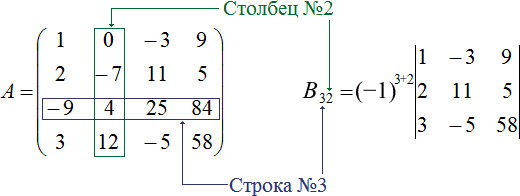
\includegraphics{im3.png}
   \caption{Вычисления алгебраического дополнения для произвольной матрицы}
   \label{im3}
\end{figure}


\subsection{Метод распараллеливания алгоритма}
При распараллеливании алгоритма каждое алгебраическое дополнение для строки $i$ и столбца $j$ считается на отдельном потоке. Для этого в функции запуска ядра каждому потоку выдаются свои значения $i$ и $j$ в соответствии с его номером. Номер потока вычисляется следующим образом: 
$$threadId = threadIdx.x + blockIdx.x * blockDim.x$$ 
где threadIdx.x - номер потока в блоке по оси x, 
blockIdx.x - номер блока по оси x,
blockDim.x - количество потоков в блоке по оси x.

Чтобы упростить работу с матрицами, они были представлены в виде векторов. Чтобы получить доступ к определенному элементу этого вектора, происходит преобразование столбцов и строк матрицы в линейный индекс:

$$index=row * cols + col$$
где index - конечный индекс элемента в векторе,
row - номер строки в матрице,
col - номер столбца в матрице,
cols - количество столбцов в матрице. 

Чтобы перейти от индексации вектора к индексации матрицы, производятся следующие преобразования:
$$row= \frac{index}{cols}$$
$$col=index \hspace{2mm} mod \hspace{2mm} cols,$$
где index - конечный индекс элемента в векторе,
row - номер строки в матрице,
col - номер столбца в матрице,
cols - количество столбцов в матрице.

По этим двум формула происходит выделение индексов  $i$ и $j$, по которым будут убраны строка и столбец. 

Чтобы поток мог произвести повторные вычисления, если потоков недостаточно для полного покрытия матрицы, то происходит смещение по следующий формуле:
$$threadId = threadId + blockDim.x * gridDim.x$$
где threadId - номер потока в блоке по оси x, 
blockDim.x - количество потоков в блоке по оси x,
gridDim.x - количество потоков по оси x.

После вычисления алгебраического дополнения поток записывает его в матрицу $n \times n$ в строку $i$ и в столбец $j$. 

\newpage
\section{Описание эксперимента}

В этом разделе выполняется исследование времени решения задачи при изменении следующих параметров:
\begin{itemize}
    \item Размеры матрицы: $32 \times 32$, $75 \times 75$, $100 \times 100$;
    \item Количество блоков: 1, 10, 100, 1000, 10000;
    \item Количество потоков: 1, 10, 100, 1000;
    \item Используемая память: глобальная, глобальная и константная.
\end{itemize}

Для измерения времени вычислений использовался модуль time.h. 

Измерение происходило следующим образом:
\begin{enumerate}
    \item Происходила генерация матрицы;
    \item Выделение данных для host;
    \item Запись времени начала эксперимента;
    \item Инициализация памяти на device;
    \item Проведение вычислений;
    \item Очистка памяти;
    \item Запись времени конца эксперимента;
    \item Вывод разницы между временем начала эксперимента и его конца.
\end{enumerate}

\newpage
\section{Анализ результатов}

В таблицах 1, 2, 3 приведены результаты измерения времени в милисекундах для глобальной памяти для размеров матрицы $32 \times 32$, $75 \times 75$, $100 \times 100$ соответственно. Знаком --- отмечены те случаи, при которых произошла нехватка памяти. В таблицах 4, 5, 6 приведены результаты измерения времени в милисекундах для глобальная и константная памяти для размеров матрицы $32 \times 32$, $75 \times 75$, $100 \times 100$ соответственно.

\begin{table}[H]
    \centering
    \caption{Результаты измерения времени исполнения программы для матрицы $32 \times 32$ и глобальной памяти}
    \footnotesize
    \begin{tabularx}{\textwidth}{|X|X|X|X|X|X|}
    \hline
    \textbf{Числов блоков в потоке} & \multicolumn{5}{|c|}{\textbf{Число блоков}} \\ 
    \hline
    &  1&	10&	100&	1000&	10000 \\
    \hline
    1 & 4440	& 450	& 50 & 	20 & 	20\\
    \hline
    10 & 	900 &	100 &	40 &	10 &	20\\
    \hline
    100	& 210 & 60	& 30	& 50	& 40\\
    \hline
    1000 &	120 &	100	& 120 &	110 & 	100\\
    \hline
    \end{tabularx}
\end{table}

\begin{table}[H]
    \centering
    \caption{Результаты измерения времени исполнения программы для матрицы $75 \times 75$ и глобальнной памяти}
    \footnotesize
    \begin{tabularx}{\textwidth}{|X|X|X|X|X|X|}
    \hline
    \textbf{Числов блоков в потоке} & \multicolumn{5}{|c|}{\textbf{Число блоков}} \\ 
    \hline
    &  1&	10&	100&	1000&	10000 \\
    \hline
    1	& 217020	& 22110	& 2380& 	1080	& 940\\
    \hline
    10	& 44810	& 4610	&---	&---	&---\\
    \hline
    100&	10140&	---	&---&	---&	---\\
    \hline
    1000&	4630&	---&	---&	---&	---\\
    \hline
    \end{tabularx}
\end{table}

\begin{table}[H]
    \centering
    \caption{Результаты измерения времени исполнения программы для матрицы $100 \times 100$ и глобальнной памяти}
    \footnotesize
    \begin{tabularx}{\textwidth}{|X|X|X|X|X|X|}
    \hline
    \textbf{Числов блоков в потоке} & \multicolumn{5}{|c|}{\textbf{Число блоков}} \\ 
    \hline
    &  1&	10&	100&	1000&	10000 \\
    \hline
    1	&1187990	&119440	&11950&	5860&	5060\\
    \hline
    10	&245640	&24780   &	---&	---	&---\\
    \hline
    100&	62360 &	---	&---	&---&	---\\
    \hline
    1000&	---&	---	&---	&---&	---\\
    \hline
    \end{tabularx}
\end{table}

\begin{table}[H]
    \centering
    \caption{Результаты измерения времени исполнения программы для матрицы $32 \times 32$ и глобальная и константная памяти}
    \footnotesize
    \begin{tabularx}{\textwidth}{|X|X|X|X|X|X|}
    \hline
    \textbf{Число блоков в потоке} & \multicolumn{5}{|c|}{\textbf{Число блоков}} \\ 
    \hline
    &  1&	10&	100&	1000&	10000 \\
    \hline
    1&	4030&	390&	50	&20	&20\\
    \hline
    10&	840&	100	&20	&20&	20\\
    \hline
    100&	220&	50&	50&	40&	50\\
    \hline
    1000&	110&	110&	110& 100&	110\\
    \hline
    \end{tabularx}
\end{table}

\begin{table}[H]
    \centering
    \caption{Результаты измерения времени исполнения программы для матрицы $75 \times 75$ и глобальная и константная памяти}
    \footnotesize
    \begin{tabularx}{\textwidth}{|X|X|X|X|X|X|}
    \hline
    \textbf{Число блоков в потоке} & \multicolumn{5}{|c|}{\textbf{Число блоков}} \\ 
    \hline
    &  1&	10&	100&	1000&	10000 \\
    \hline
    1&	200490&	20310&	2070&	990&	860\\
    \hline
    10&	43150&	4420&	---&	---&	---\\
    \hline
    100&	10380&	---&	---&	---&	---\\
    \hline
    1000&	4560&	---&	---&	---&	---\\
    \hline
    \end{tabularx}
\end{table}

\begin{table}[H]
    \centering
    \caption{Результаты измерения времени исполнения программы для матрицы $100 \times 100$ и глобальная и константная памяти}
    \footnotesize
    \begin{tabularx}{\textwidth}{|X|X|X|X|X|X|}
    \hline
    \textbf{Число блоков в потоке} & \multicolumn{5}{|c|}{\textbf{Число блоков}} \\ 
    \hline
    &  1&	10&	100&	1000&	10000 \\
    \hline
    1&	1101650&	111320&	11190&	5500&	4730\\
    \hline
    10&	237750&	24120&	---&	---&	---\\
    \hline
    100&	56750&	---&	---&	---&	---\\
    \hline
    1000&	---&	---&	---&	---&	---\\
    \hline
    \end{tabularx}
\end{table}


Как можно увидеть, что при максимальном количестве блоков вычисление алгебраических дополнений матрицы показываются минимальный показатель затраченного времени, но увеличении потоков время выполнения возрастает. Это происходит из-за того, что выделено слишком большое число потоков, которые не выполняют никаких вычислений. 

Из роста количества потоков видно, что при их большом количестве время возрастает даже для одного блока. Таким образом, можно сделать вывод, что произведение числа блоков на число потоков должно быть приблизительно равно количеству элементов в матрице. При этом мы получим самое минимальное время, если количество блоков будет больше, чем количество потоков.

Были выделены лучшие конфигурации для матриц с разными размерами:
\begin{itemize}
    \item Для матрицы с размером $32 \times 32$ - 1000 блоков, 100 потоков;
    \item Для матрицы с размером $75 \times 75$ - 10000 блоков, 1 поток;
    \item Для матрицы с размером $100 \times 100$ - 10000 блоков, 1 поток;
\end{itemize}

Для константной памяти время вычисления меньше, чем время вычисления без нее, но на небольшую долю. В среднем время выполнения при использовании глобальной памяти больше время выполнения при использовании глобальной и константной памяти на 5\%. 

Также появляется одна проблема. При больших размерах исходной матрицы($75 \times 75$ и $100 \times 100$) и потоков на одном блоке происходит нехватка памяти. Дело в том, что каждая такая матрица копируется внутри каждого потока, и при большом количестве потоков в блоке не хватает памяти.

На Рис. \ref{im4} отображена зависимость времени от разного числа потоков в определенной выборке блоков.

\begin{figure}[H]
   \centering
   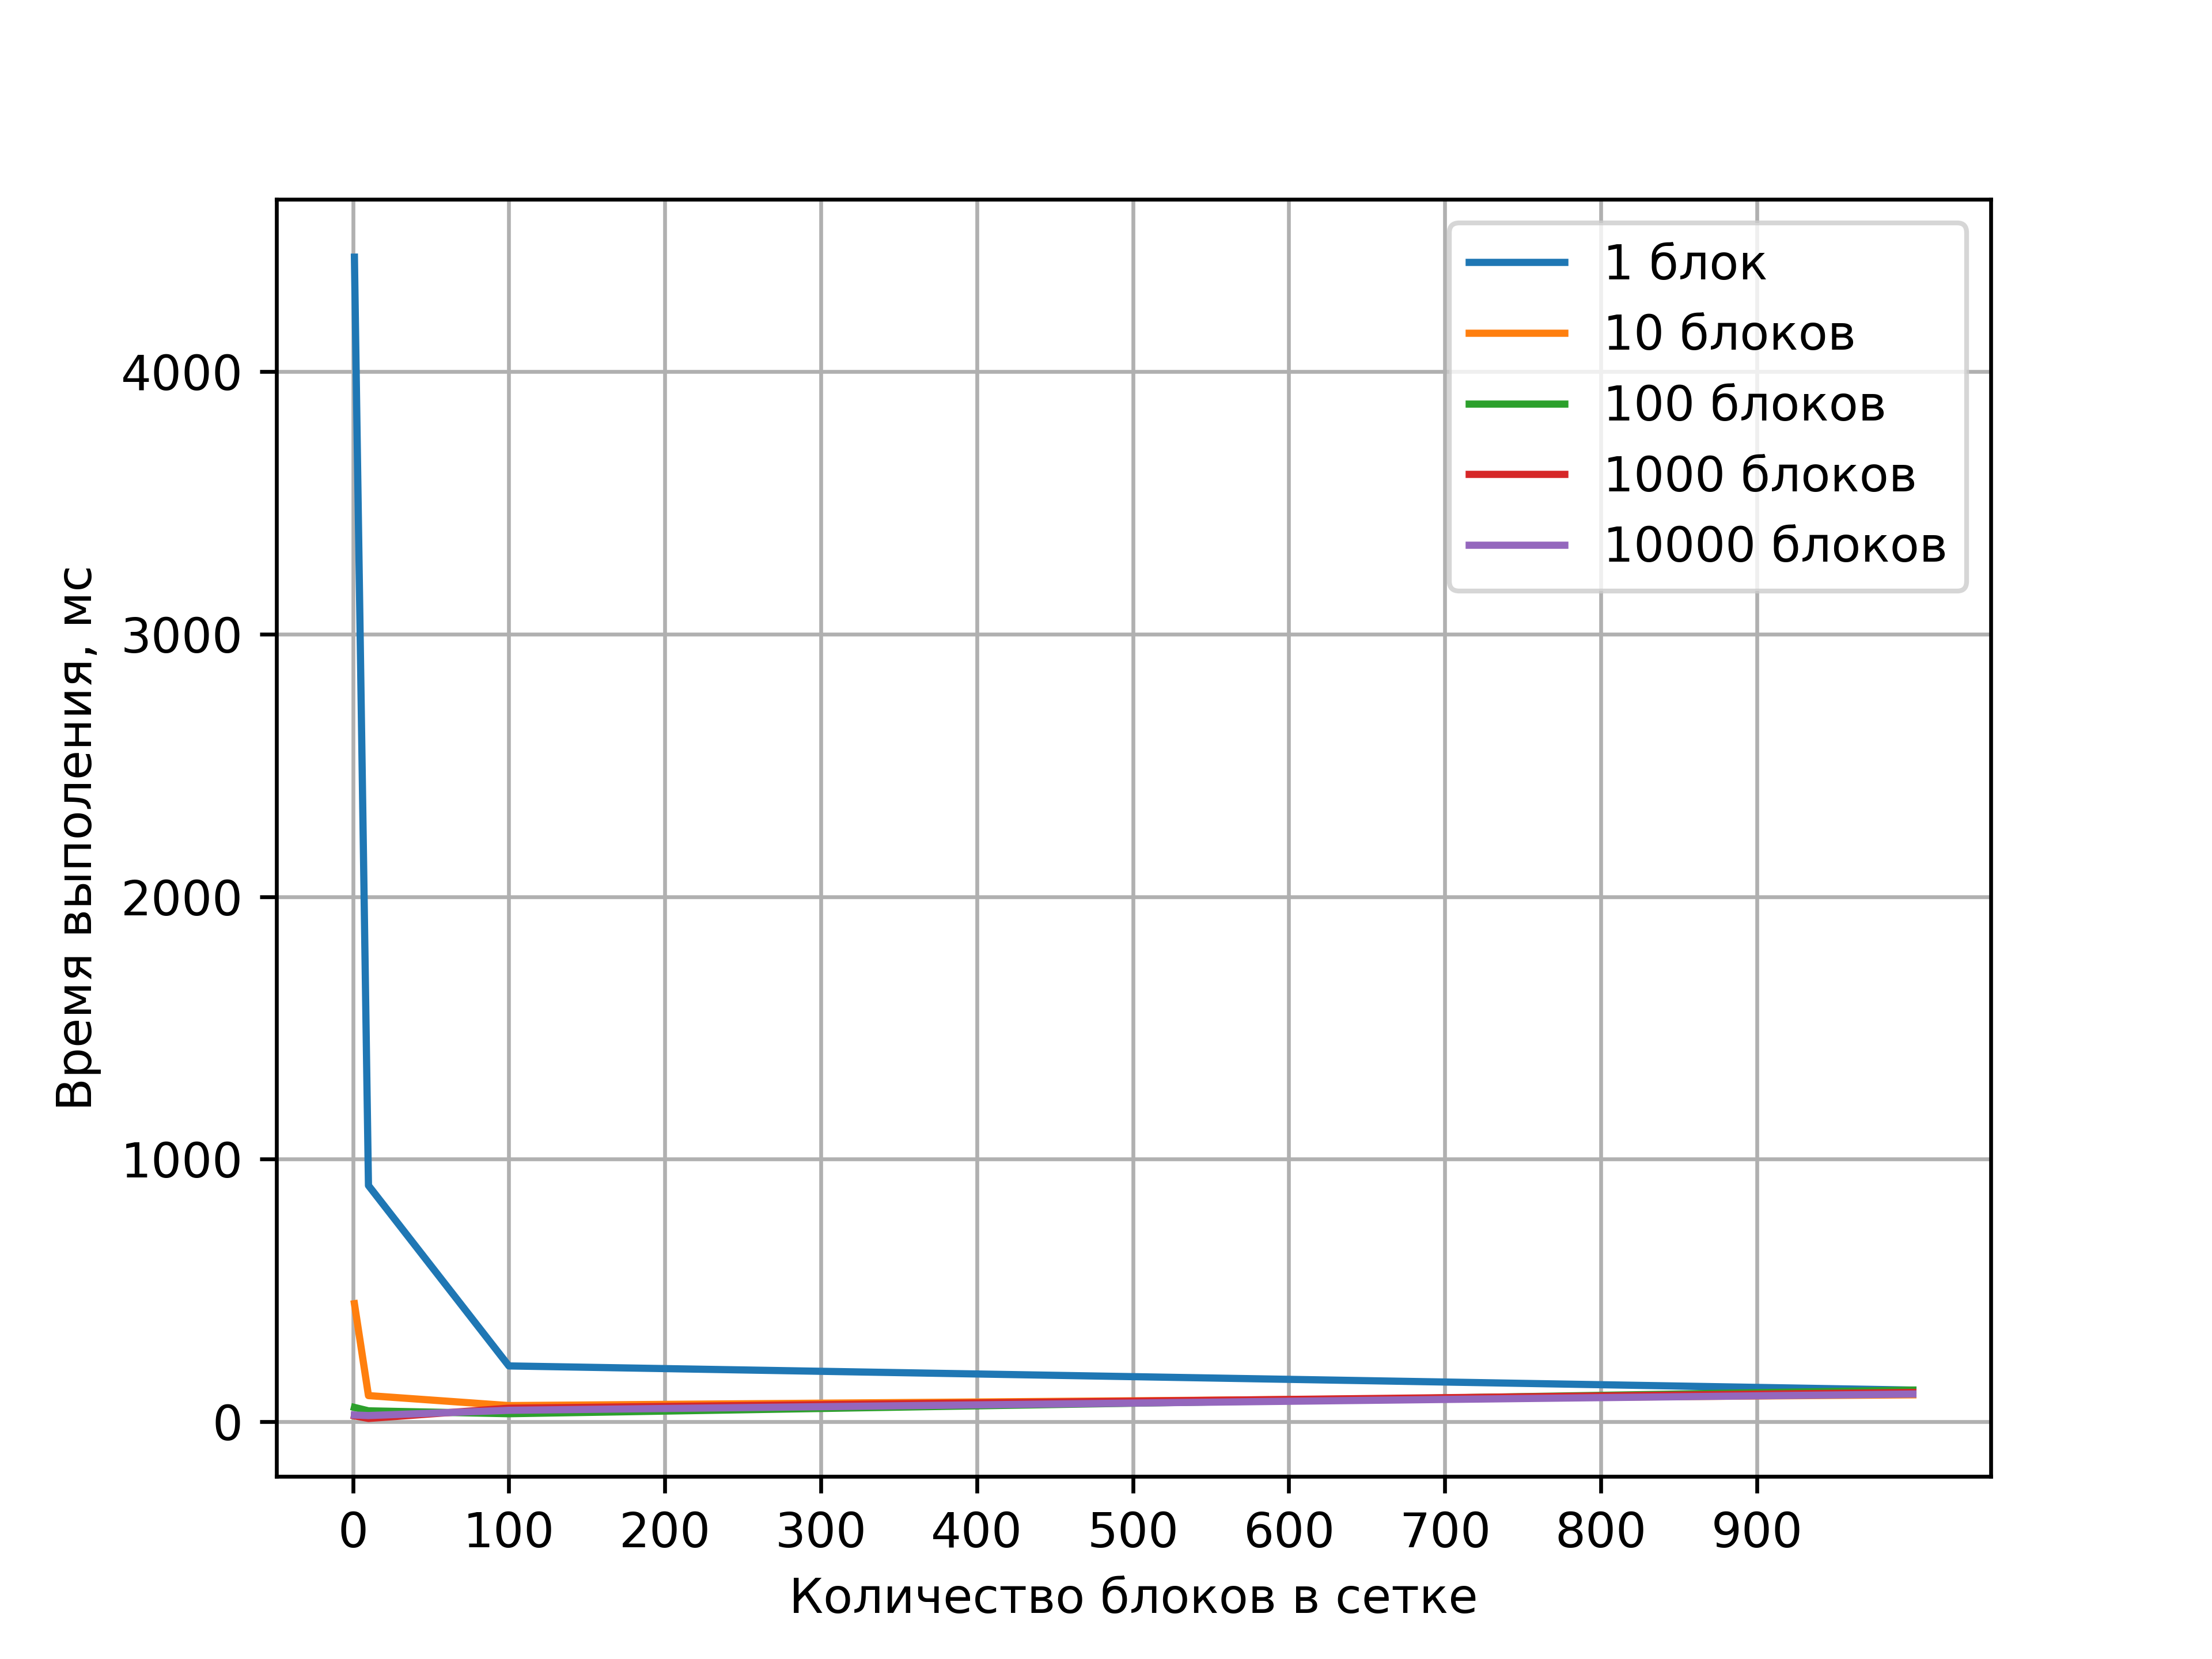
\includegraphics[width=1.0\linewidth]{im4.png}
   \caption{Зависимость времени от разного числа потоков в определенной выборке блоков}
   \label{im4}
\end{figure}

\newpage
\section*{Заключение}
\addcontentsline{toc}{section}{Заключение}
В рамках курсовой работы было изучена технология параллельного программирования
на основе архитектуры Nvidia CUDA.

Для задачи подсчета фигур на изображении был разработан параллельный асинхронный
алгоритм, алгоритм был реализован на языке CUDA C. Программа была запущена на
ресурсах суперкомпьютерного центра «Политехнический». Для запуска использовался
узел типа «Торнадо» с видеокартой NVIDIA Tesla K40X. Запуск программы проводился
на одном узле с использованием одной видеокарты.

Для программы было измерено время работы при различной степени распараллеливания. Полученные результаты согласовались с теоретической оценкой максимального
количества потоков. Использование оптимальной конфигурации позволило уменьшить
время выполнения в 400 раз относительно наихудшей конфигурации для матрицы $32 \times 32$, в 230 раз для $75 \times 75$ и в 235 раз для $100 \times 100$.

Реализация алгоритма с использованием константной памяти увеличило время выполнение в среднем на 5\%.

Измерение времени исполнения в зависимости от размера матрицы показало линейную
зависимость.

В рамках курсовой работы была написана программа размером около 300 строк. Работа на
СКЦ «Политехнический» шла три недели, за это время было сделано примерно 50 авторизаций и порядка 100 запусков задач на исполнение.

Для сборки использовался компилятор NVCC версии 11.6u2.


\newpage
%Список источников
\begin{thebibliography}{0}
	
\bibitem{cuda_tech} Эдвард Кэндрот, Джейсон Сандерс <<Технология CUDA в примерах. Введение в программирование графических процессоров>> -- ДМК-Пресс, 2018 г. -- 232 c.
        \bibitem{cuda_guide} CUDA Programming Guide 12.1 (\url{http://developer.download.nvidia.com/compute/cuda/1_1/NVIDIA_CUDA_Programming_Guide_1.1.pdf}).
        \bibitem{scc} Краткое руководство пользователя вычислителей «Политехник - РСК Торнадо» и «Политехник - РСК Петастрим».
    


\end{thebibliography}
\addcontentsline{toc}{section}{Список источников}


\end{document}